%!TEX program = xelatex 
\documentclass[a4paper,zihao=-4]{article}
\usepackage[UTF8,punct,linespread=1.56]{ctex}
% \documentclass[a4paper,cs4size,UTF8,punct,linespread=1.56]{ctexart}
\pagestyle{empty} % 第二页以后页码空白
\usepackage[a4paper, left = 3.2cm, right = 3.2cm, top = 2.54cm, bottom = 2.54cm]{geometry}
\usepackage{xcolor}
% \usepackage[citebordercolor = white]{hyperref}
\usepackage[hidelinks]{hyperref}
\usepackage{graphicx} 
\usepackage{amsmath}
\usepackage{amssymb}
\usepackage{times}
\usepackage{float}
\usepackage{multirow}
\usepackage[subrefformat=parens,labelformat=parens]{subfig} %
\usepackage{booktabs} % for \toprule \midrule \bottomrule \cmidrule
\usepackage{cleveref}
\crefformat{table}{表~#2#1#3}
\crefformat{figure}{图~#2#1#3}
\crefformat{equation}{式~（#2#1#3）}
\usepackage{enumitem}
% \setenumerate[1]{itemsep = 0pt, parsep = 0pt, topsep = 2bp}
\setlist[enumerate]{itemsep = 0pt, parsep = 0pt, topsep = 2bp}
% \setitemize[1]{itemsep = 0pt, parsep = 0pt, topsep = 2bp}
\setlist[itemize]{itemsep = 0pt, parsep = 0pt, topsep = 2bp}
\usepackage{fontspec}
\setmainfont{Times New Roman}
% \usepackage{minted}   % For syntax highlighting
% \usemintedstyle{friendly}
\usepackage{setspace} 
\usepackage{caption}
\DeclareCaptionFont{capfont}{\kaishu\zihao{-4}\selectfont} % Caption font
\DeclareCaptionFont{subfont}{\kaishu\zihao{5}\selectfont} % Sub-caption font
\captionsetup{font = capfont}
\captionsetup[subfigure]{font = subfont}
\captionsetup[figure]{labelsep=space} % 空格 space；点 period；冒号 colon
\captionsetup[table]{labelsep=space}  % 空格 space；点 period；冒号 colon
\usepackage[square,numbers,sort&compress]{natbib}   % For Reference
\newcommand{\citess}[1]{\textsuperscript{\cite{#1}}}
\setlength{\bibsep}{1pt plus 0.3ex}
\usepackage{titlesec}
\titleformat{\subsubsection}[block]{\hspace{3em}}{\thesubsubsection}{1em}{}
\usepackage{insfc}



\graphicspath{{images/}}   % 设置图片所存放的目录

\begin{document}

\kaishu

% Decrease space above and below equations
\setlength{\abovedisplayskip}{0pt}
\setlength{\belowdisplayskip}{0pt}

%%%%%%%%% TITLE %%%%%%%%%
% \title{报告正文 \vspace{-3.4ex}}
% \title{报告正文}
% \maketitle
\begin{center}
	{\kaishu \zihao{2} \textbf{报告正文} \vspace{-3ex}}
\end{center}  

\thispagestyle{empty} 　　　% 首页页码空白

%%%%%%%%% Your Content %%%%%%%%%
{\kaishu \zihao{4}参照以下提纲撰写，要求内容翔实、清晰，层次分明，标题突出。}\alert{请勿删除或改动下述提纲标题及括号中的文字。\vspace{9bp}}

\NsfcChapter{\textbf{（一）立项依据与研究内容}}{（建议8000字以内）；}

\NsfcSection{1}{项目的立项依据}{（研究意义、国内外研究现状及发展动态分析，需结合科学研究发展趋势来论述科学意义；或结合国民经济和社会发展中迫切需要解决的关键科技问题来论述其应用前景。附主要参考文献目录）；}

\subsection{研究意义}

我国在《国家中长期科学和技术发展规划纲要（2006-2020）》中，将地质灾害遥感调查与监测技术列为公共安全重点领域及优先主题。
我国当前经济社会处于高速发展时期，人类工程活动（如基础建设、水利工程、毁林开荒等）诱发的地质灾害呈现逐年增加的趋势。
因此，在未来几十年，我国地质灾害防治工作任务艰巨。发展实时性强、监测范围广的地质灾害遥感监测与评估技术，符合当前我国社会经济发展的重大战略需求。

三峡库区地质灾害受降雨的影响极为严重，每年都会发生降雨诱发滑坡，严重威胁库区人民的人身财产安全。
开展近实时降雨条件下的滑坡危险性评价研究，对于防灾减灾，保障三峡大坝安全，保障长江航道安全，具有重要的战略意义。

依托遥感云平台海量的遥感影像、强大的运算能力和近实时更新的影像数据，使得开展面向三峡库区全区的滑坡危险性近实时动态评价成为可能。
开展基于云平台的滑坡灾害危险性评价，既是顺应时代的发展，积极拥抱新技术的体现，也是对现有滑坡危险性评价方法系统的有益补充。
因此，发展基于遥感大数据的地质灾害危险性评价技术有望提升我国的灾害管理水平，对我国的科技创新起到带动作用。

\subsection{国内外研究现状}

\subsubsection{滑坡易发性评价研究现状}

滑坡灾害是一种常见的地质现象，往往会造成大量的经济损失和人员伤亡，劣化土壤，损坏植被和房屋，甚至严重阻塞运输线路和水路\cite{Saro2016,Akgun2007,Zou2017}。
据中国地质调查局报告，2019年全国发生了6181起地质灾害，包括滑坡、塌方、泥石流、地面塌陷、地面裂缝和地面沉降等，导致211人死亡，13人失踪，75人受伤，直接经济损失高达27.7亿元。
其中，发生了4020起滑坡，主要分布在中国西南部，造成了更多的人员失踪和更严重的经济损失。
因此，开展滑坡易发性和危险性研究来减少山体滑坡造成的人员伤亡和经济损失具有重要的现实意义。

滑坡易发性评价是滑坡灾害管理的基础，其评价结果表示基于历史滑坡和相关因素的给定区域内滑坡发生可能性的空间分布\cite{pourghasemi2018analysis,Song2018,Yu2016_GWR_SVM}。
影响滑坡发生的因素可以分为“控制因素”（地貌、水文、岩性和植被覆盖等）和“诱发因素”（降雨、库水位波动和人类工程活动等）\cite{Rabby2020,Arabameri2020}。
因此，获取影响滑坡发生的因素并采用适当的建模方法是滑坡易发性评价的基础。在滑坡易发性评估研究中，发展出了各种确定性或非确定性的方法和技术，并取得了显著的进展\cite{Yu2016_GWR_SVM,Xu2016}。确定性方法包括专家系统方法\cite{Zhu2014AnLSM_fuzzy_logic}、模糊逻辑\cite{Aksoy2012,Anbalagan2015,Shahabi2015RemoteLSM_fuzzy_logic,Roy2019a,Reichenbach2018,Pradhan2011UseLSM_fuzzy_logic,Amirahmadi2016,Kumar2015}、层次分析法\cite{Yoshimatsu2006,Hung2015,Yalcin2011}等；早期的非确定性方法则主要基于概率统计模型，例如信息量法\cite{chen2016comparison_LSM_INFORVALUE}、证据权法\cite{Ozdemir2013ALSM_FR_WE_LR}和频率比法\cite{Goetz2015}等。

如今，随着计算机技术以及遥感、地理信息系统技术的飞速发展，大量基于机器学习算法的非确定性方法被广泛应用到了滑坡易发性评价当中。一些研究人员已经基于地理信息系统和遥感技术应用不同的机器学习模型来评估滑坡易发性，其中包括逻辑回归\cite{Bai2010,ayalew2005application,Yilmaz2009,Akgun2012LSM_LR_MCD_FR,Yesilnacar2005,Eeckhaut2006,Lee2007LSM_FR_LR_ANN,Chauhan2010LSM_LR}、人工神经网络\cite{Lee2020,Ghorbanzadeh2019,2010Landslide}和支持向量机\cite{Othman2014,Adnan2020,Dou2019,Shao2019}等。
集成学习方法（Ensemble Learning）是传统机器学习模型的一种改进，使用多个弱分类器联合形成一个强分类器。
集成学习在许多实际学习任务中比传统的机器学习方法表现出更强的性能，并且已在滑坡易发性评价当中得到了广泛使用\cite{Kadavi2018,Adnan2020,Napoli2020}。
其中，随机森林（Random Forest, RF）是集成学习方法中Bagging方法的扩展变体\cite{Breiman2001}，具有实现简单、计算开销低的优势，也被广泛应用到了滑坡易发性评价当中\cite{Youssef2015,Pourghasemi2016,Kim2017}。 

但是，在给定的研究区域中，滑坡样本通常比非滑坡样本少得多。以往基于机器学习模型的滑坡易发性评价研究在进行非滑坡样本选取时往往采用随机选点的方法，即选择与滑坡样本数量相当的非滑坡样本，共同组成滑坡易发性评价的类别标签数据。这种处理方法一方面会造成非滑坡样本的浪费和重要信息的丢失；另一方面，随机选取少量的非滑坡样本无法代表研究区非滑坡样本的分布情况，与机器学习中“训练集是真实样本总体的无偏估计”前提相背离，影响所构建模型的性能，导致所构建的模型泛化能力差。

本研究拟在进行易发性评价中，针对不同类别（滑坡，非滑坡）设置不同的误分类权重，即“类别加权”。类别加权算法已被广泛用于解决类别不平衡问题，但在滑坡易发性分析中的应用仍然较少。本研究将易发性评价问题看作一个类别不均衡的机器学习问题，将“类别加权”引入到随机森林方法当中，对传统随机森林方法进行改造，使之适用于处理类别不均衡问题。

\subsubsection{区域尺度滑坡危险性评价研究现状}

评估区域到全球尺度的滑坡灾害危险性动态变化的研究还比较少。Hong等于2006年提出了第一个准全球近实时滑坡危险性评价系统\cite{Hong2006}。
该系统将TRMM降雨数据与全球滑坡易发性分区结果结合在一起，评估了全球滑坡的危险性。
一些研究者静态地描述了大区域尺度的滑坡灾害\cite{Nadima2009},或随着时间的推移发生的变化\cite{Farahmand2013}，但不能定期或近乎实时地获取信息。
区域滑坡灾害管理突出了利用遥感源对滑坡灾害或早期预警进行动态描述\cite{Rossi2012,Kirschbaum_2015_Dynamic,Liao2011}，这些研究受制于当地的地形地貌条件、滑坡调查数据和降雨数据的可用性，限制了其在其他地区的推广和应用。
数据的日益开放和地理空间工具的进步，包括地理信息系统、商业和免费图像处理软件，高级编程语言以及云计算和机器学习，增加了更好地利用地球观测数据进行滑坡测绘和灾害评估的可能性。然而，融合多个遥感数据源，以便以易于获取、快速传播和简明易懂的方式表征滑坡灾害，仍然是一个值得深入研究的课题。

动态滑坡灾害评估的方法在很大程度上取决于公众的需求、地理区域和所考虑的空间尺度。
降雨是世界上最普遍和频繁发生的山体滑坡的诱发因素\cite{Kirschbaum_2015_Dynamic}，因此，有效地表征与降雨相关的触发模式是国际地质灾害研究领域的热点问题。
然而，基于季节性、地理和气候学的降雨量变化很大\cite{Guzzetti2007}，降雨与降雪会使得土壤湿度发生改变，加上人类工程活动的影响，使得确定降雨阈值变得复杂。滑坡的易发性也会受地形的制约，但这些信息的准确性和可用性因地区而异。
滑坡的发生可以看作控制因素（也被称为本底因素\cite{滑坡⻛险区划理论与实践}）与诱发因素共同作用的结果。
动态指的是区域上具有一定地域性动态变化的诱发条件，如库水位变动、人类工程活动、潜在的崩塌冲积加载和一般的降雨过程等方面。关于滑坡危险性的动态评估，来自NASA的研究人员Kirschbaum等于2015年提出了Landslide Hazard Assessment for Situational Awareness（LHASA）模型，使用近实时的GPM降水数据结合世界范围的滑坡易发性分区图，实现了中美洲和加勒比群岛的滑坡的近实时预警\cite{Kirschbaum_2015_Dynamic}。
考虑降雨的滑坡动态评价的关键之处在于降雨阈值的选择，即研究导致边坡失稳的降雨阈值，作为滑坡危险性预报预测的评判标准。
所谓阈值，即某个过程发生或开始变化所需的某个量的最值。
对于滑坡来说，阈值可以是土壤含水量、降雨强度、孔隙水压力等水文地质条件，当达到阈值，可以认为滑坡有可能发生。Kirschbaum等使用了60日累积降雨量和当日降雨量作为判别因子，采用降雨数据的百分位数作为降雨阈值\cite{Kirschbaum_2015_Dynamic}。

区域滑坡危险性评价是国内国际的研究热点，开展区域性滑坡危险性评价也是提升我国灾害管理水平、防灾减灾、保障人民生命财产安全的必由之路。许多项目和研究都提出了天地一体化、空天地一体化的概念，将卫星遥感数据、航空遥感数据、地质调查数据等应用到了滑坡易发性和滑坡危险性评价当中，体现了多源数据融合和学科交叉的思想。

然而，目前这方面的研究还存在一些不足，数据的获取比较困难，数据的处理过程往往会花费大量的时间。此外，一些研究往往随着项目的结题而终止，研究成果不具备推广性和时效性。

\subsubsection{遥感大数据云平台研究现状}

随着大数据技术和云存储技术的发展，Google Earth Engine（以下简称GEE）、NASA Earth Exchange、AWS、TerraLib、Hadoop、GeoSpark、GeoMesa、Microsoft Azure和地质云等云平台应运而生，为大规模的遥感应用和地理空间分析提供了新的视角和机遇\cite{Hird2017}。
地理数据云平台的出现为构建具有高时效性、高持续性和可推广性的滑坡危险性评价系统提供了必要条件。

不同于TerraLib、GeoSpark和GeoMesa等大规模地理空间数据处理工具，GEE无需掌握复杂的编程语言和编程技能，简单的脚本语言（Python或者JavaScript）和相对简单的语法即可满足要求。
GEE为研究人员提供了强大的运算能力，使得遥感数据的分析与处理变得更加的高效，为区域尺度甚至全球尺度的地理空间分析研究提供了一种有效的途径\cite{Tamiminia20_Google}。
GEE的发展，能够使研究人员能够将更多的精力放在算法和模型的开发上，大大地促进了其在地理空间分析和遥感应用中的发展\cite{Tamiminia20_Google}。
不同于AWS和Microsoft Azure，GEE作为免费的遥感大数据学习平台，为研究人员提供了很好的学习模式\cite{Amani20_Google}。
通过这个平台，研究人员能够在短时间内实现大尺度区域的研究。进而让研究人员可以有更多的时间去开发能够应用于自己研究领域的大尺度和全球化的应用算法。
GEE公共数据目录是包含了PB级的地理空间数据集，该目录的大部分数据由对地观测的遥感影像组成，包括整个Landsat系列以及Sentinel-1和Sentinel-2的完整数据，另外它还包括气候预测，土地覆盖数据，地球物理和社会经济数据集及和许多其它环境数据等\cite{Tamiminia20_Google}。
该目录以每天近6000景的速度进行更新。当前通过GEE应用平台,能够实现海量地球科学数据的访问和处理\cite{Tamiminia20_Google}。
GEE的资源管理器是一个简单的Web应用程序，用于数据目录浏览，可视化和基本分析，允许用户运行简单的分析。
同时，GEE内置了常用的机器学习方法，包括逻辑回归，支持向量机和随机森林等\cite{Tamiminia20_Google}。

地理大数据的激增以及云计算和大数据处理服务的最新进展正在改变遥感和地理信息系统应用的未来\cite{Amani20_Google}。
在这方面，GEE正在有效地为研究人员、科学家和开发人员能够轻松地从大的遥感数据集中提取有价值的信息，而不需要传统的数据分析方法的负担。
GEE提供的大量遥感数据集（如存档的陆地卫星和哨兵图像）有助于研究人员应对全球挑战和环境问题，如全球变暖、气候变化、大面积土地利用分类以及几十年来的景观监测。
GEE还包含数百个预先构建的功能，可以方便地被不同的用户理解和使用。这些优势使得任何用户都可以将此云计算平台用于土地利用、农业、水文、自然灾害等各种应用中。
然而，GEE还存在一些局限性，比如每个用户的存储空间有限（免费空间为15GB），训练机器学习算法的内存有限，这可能会造成新用户的减少\cite{Amani20_Google}。
然而，不可否认的是，GEE提出了一种新的地理空间数据处理方法，解决了遥感研究人员面临的数据获取与处理分析的难题\cite{Amani20_Google}。

考虑到平台的易用性、云平台的价格因素、数据的覆盖度和学习成本的高低，本研究选择GEE作为滑坡易发性评价和危险性动态评价的依托平台。
在易发性评价当中，GEE作为数据源和模型构建平台。
而在滑坡危险性评价当中，GEE作为模型构建平台和可视化显示平台。


\begin{spacing}{1.3} % 行距
	\zihao{5} \songti   
	\bibliographystyle{gbt7714-nsfc}
	\bibliography{test}  
	\vspace{11bp}
\end{spacing}

\NsfcSection{2}{项目的研究内容、研究目标，以及拟解决的关键科学问题}{（此部分为重点阐述内容）；}

\subsection{研究内容}
（1）区域尺度下滑坡易发性评价中非滑坡样本选取方法研究

（2）滑坡样本类别不均衡前提下的易发性评价方法研究

（3）GEE云平台支持下的滑坡危险性动态评价方法研究

\subsection{研究目标}
（1）发展基于GEE云平台的滑坡危险性动态评价方法；

（2）改进随机森林方法，使之适于处理类别不均衡的滑坡易发性评价问题；

（3）获取三峡库区中长期滑坡易发性动态变化情况，并由此分析三峡库区滑坡易发性动态变化趋势，归纳总结三峡库区滑坡高易发性区域的控制因素和影响因素的特征，取得三峡库区滑坡高发、频发的规律性认识。

\subsection{拟解决的关键问题}
（1）区域尺度下，滑坡易发性评价中负样本的选取问题

（2）滑坡样本类别不均衡条件下，基于机器学习的滑坡易发性评价模型构建及评价指标的选取问题

（3）基于GEE遥感云平台的区域滑坡危险性动态评价系统的构建问题

\NsfcSection{3}{\textbf{拟采取的研究方案及可行性分析}}{（包括研究方法、技术路线、实验手段、关键技术等说明）；}

\subsection{研究方法}

本项目的总体研究思路是以整个三峡库区为研究对象，以实现全库区滑坡危险性近实时动态评价为研究目标，充分发挥GEE遥感云平台的优势，利用GEE平台提供的DEM数据、Landsat系列卫星数据、MODIS系列卫星数据、GMP近实时降水数据、土地利用以及植被覆盖等数据，结合已有地质调查数据，融合“3S”技术、灾害监测技术、机器学习方法等多学科理论和技术方法，基于改进的随机森林（Weighted Random Forest, WRF）方法构建滑坡易发性评价模型，得到三峡库区滑坡易发性评价结果，结合GEE云平台提供的近实时降雨数据，基于前期降雨指数法（Antecedent Rainfall Index, ARI），构建三峡库区危险性评价模型。
在此基础上，开发基于GEE遥感云平台的滑坡危险性动态评价系统，实现三峡库区滑坡危险性的近实时动态评价。

\subsection{技术路线}

项目的总体技术方案如图\ref{fig_workflow}所示：

\begin{figure*}[htb!]
	\centering  
	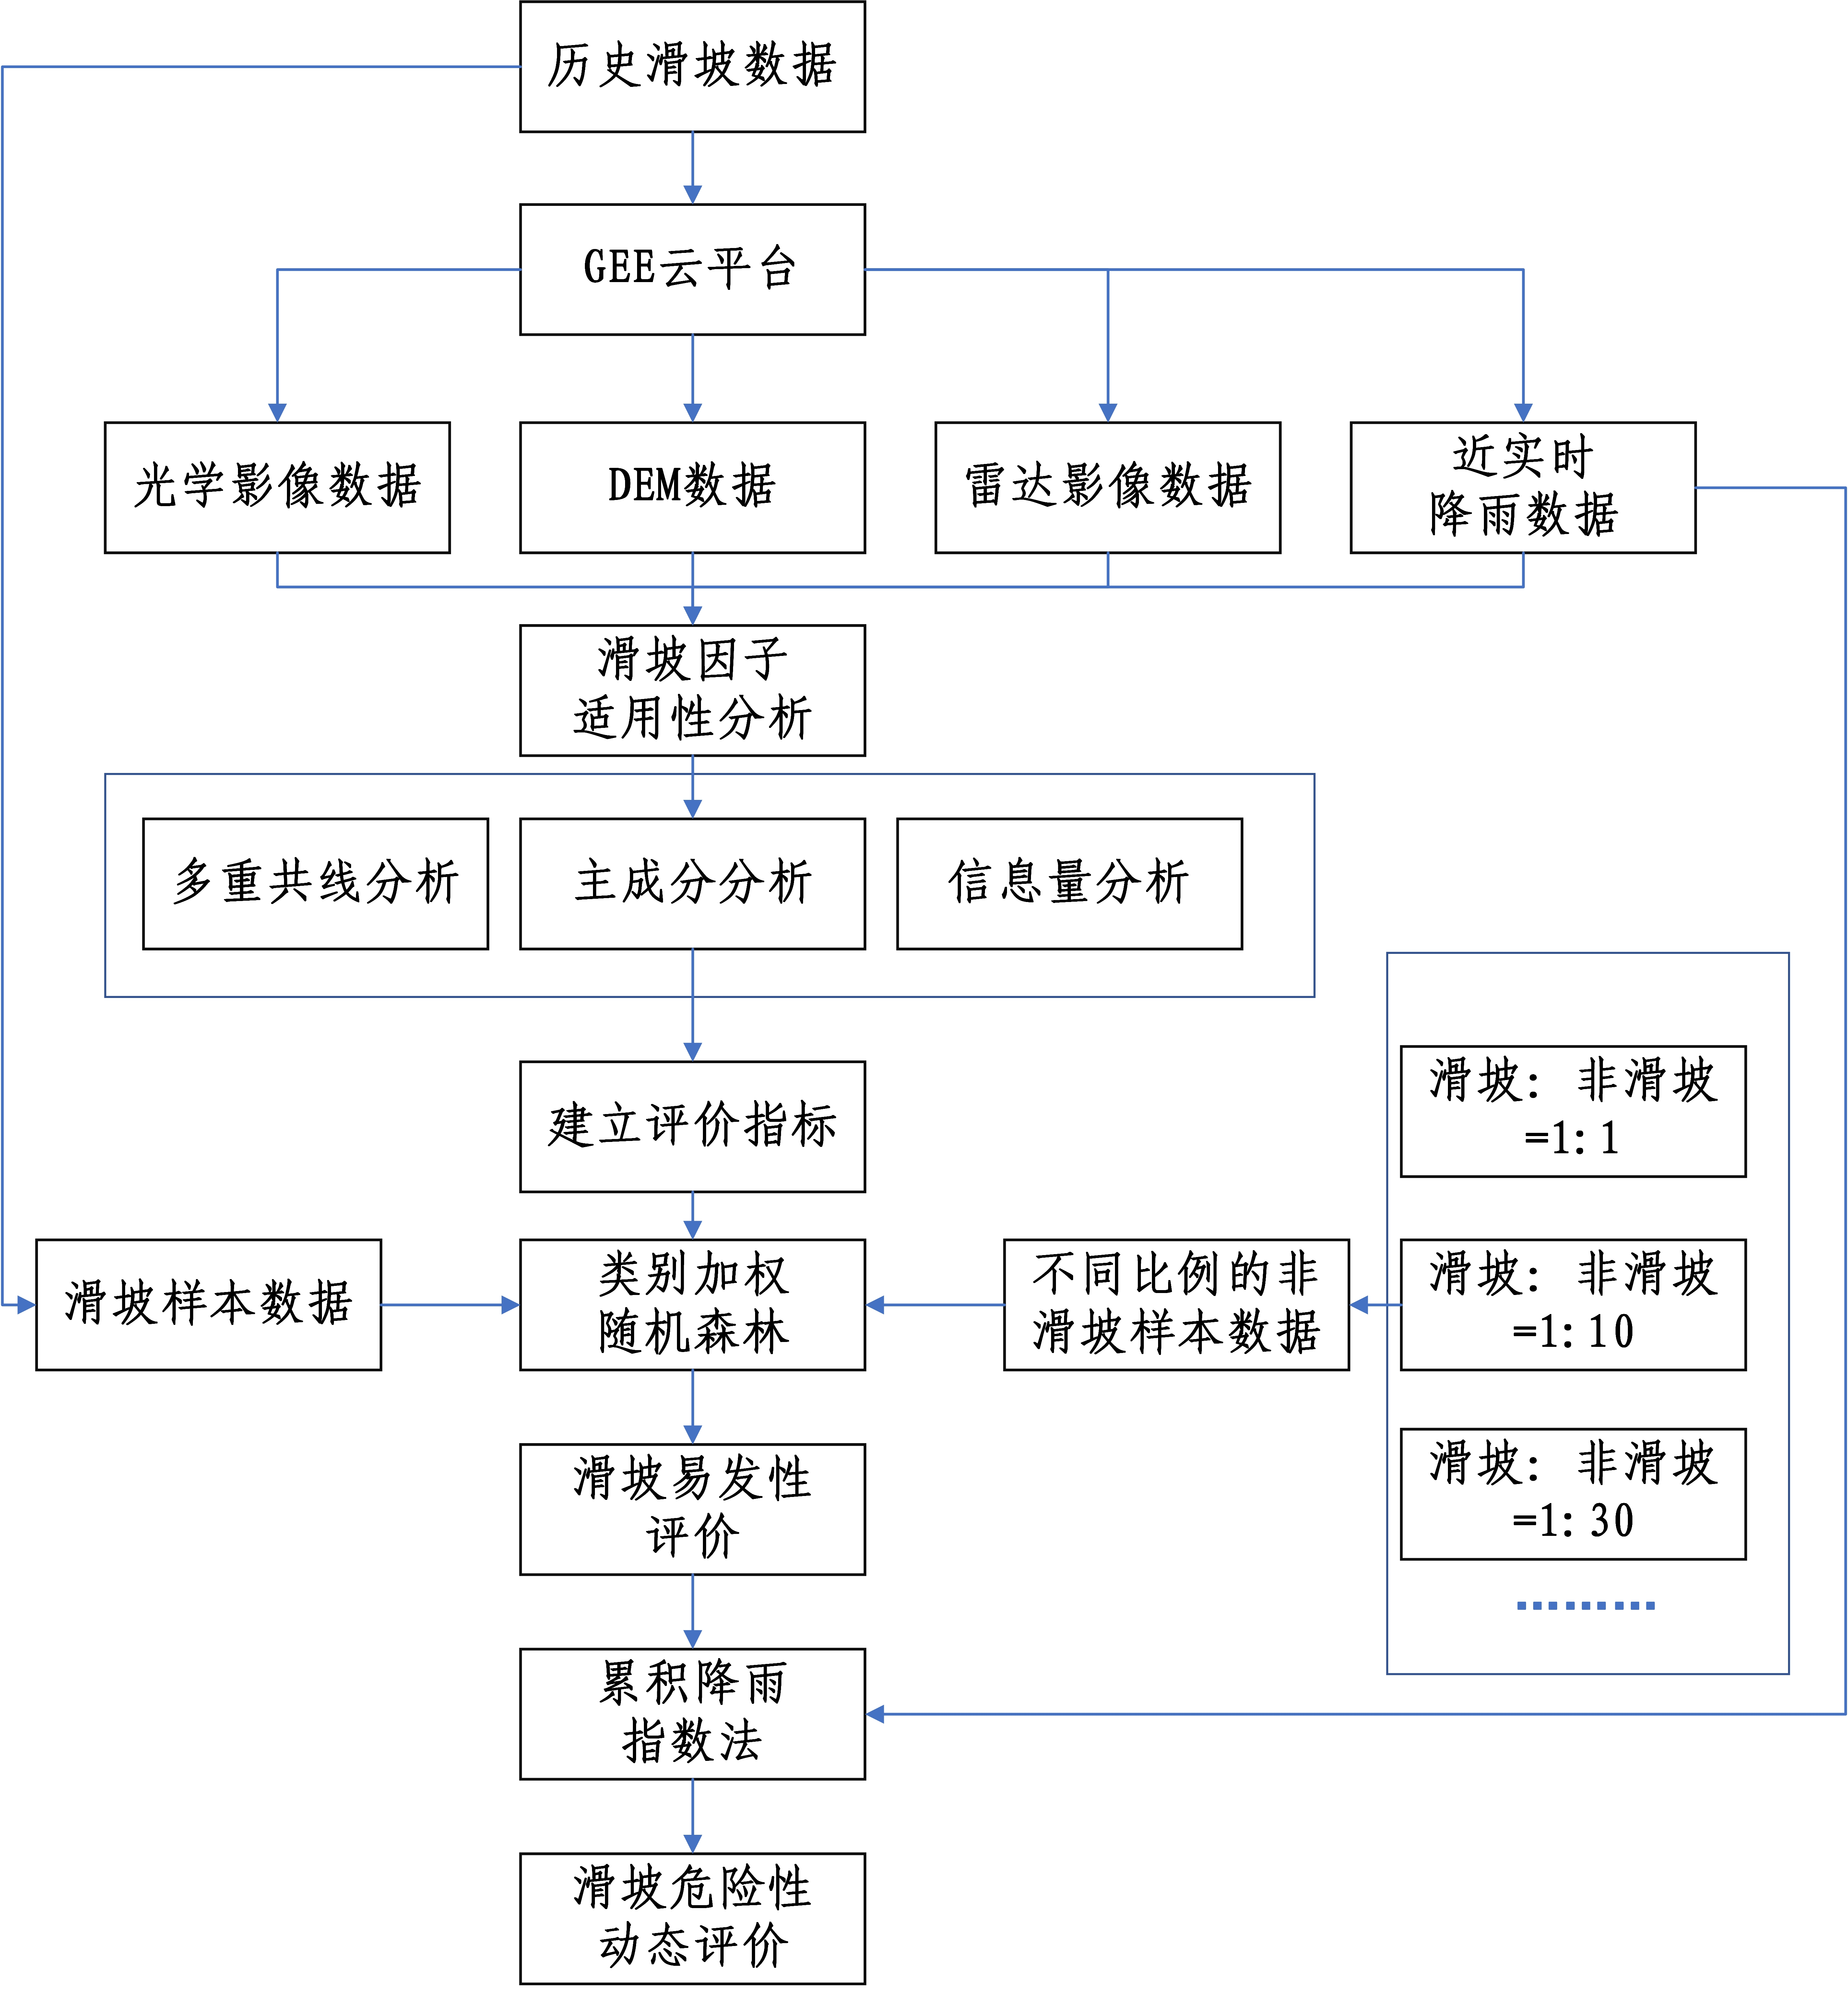
\includegraphics[width=10cm]{images/workflow4nsfc.jpg}  
	\caption{技术路线图}
	\label{fig_workflow}
\end{figure*}

\subsection{实验手段}

\subsubsection{滑坡因子获取与适用性分析}

充分利用GEE云平台提供的遥感影像，如DEM数据，Landsat系列数据等，利用GEE内置的地理空间数据处理函数，以不同的时间尺度提取坡度、坡向、地形曲率、高程等地形地貌因子以及NDVI、NDWI、TRI、TWI等地表覆盖因子，以及降水等诱发因子。将已有的滑坡地质调查数据矢量化后上传至GEE云平台，共同组成滑坡易发性评价的基础数据。

利用方差膨胀系数(variance inflation factor，VIF)、主成分分析（Principal Component Analysis，PCA）等数据预处理手段，对滑坡因子进行属性约减和因子筛选，保证易发性评价模型的健壮性。

\subsubsection{非滑坡样本的选取}

调查结果显示，三峡库区已识别的地质灾害点约5000多处，较大规模的崩滑体约2500 多处。
如果将每个矢量化后的灾害点作为一个滑坡样本，则整个库区只有5000个滑坡样本点，如果滑坡样本与非滑坡样本按照1:1的比例来选取非滑坡样本，整个研究区的样本只有10000多个，这对于建立整个库区的滑坡易发性评价模型是远远不够的。
本研究拟按照不同的样本比例来选取多份非滑坡样本，尽可能充分利用非滑坡样本，避免重要信息的丢失。然后将这些样本参与易发性评价模型的构建，并使用合适的评价指标对模型进行评价，得到合适的样本比例，为后续工作的进行打下基础。

\subsubsection{构建基于改进的随机森林方法的三峡库区滑坡易发性评价模型}

在机器学习中，随机森林是一个包含多个决策树的分类器，并且其输出的类别是由个别树输出的类别的众数而定。为了解决传统决策树易于拟合的问题，学者们将决策树算法与集成学习算法（Bagging and Boosting）相结合。随机森林方法是集成学习中Bagging家族的一员。具有简单的实现，较低的计算开销以及在许多机器学习任务中的强大性能。Bagging基础学习者的多样性不仅来自样本扰动，还来自属性扰动，这进一步提高了最终积分的泛化性能。随机森林通过替换数据和重采样来增加分类树之间的多样性，并随机更改预测集在不同的树归纳过程中的数值。

基于机器学习方法的滑坡易发性评价问题往往可以看作一个二分类问题或者回归问题看待。
然而，很少有研究关注易发性评价当中的滑坡样本不均衡的问题。理想的机器学习模型当中，样本类别往往是平衡的，意味着对应每个类别的训练样本数量大致相同。而在处理真实的、未经清洗的数据时，数据类别的不平衡现象往往是一个普遍存在的现象。
例如，每年有2\%的信用卡用户遭遇电信诈骗；磁盘驱动器故障率约为1\%等等。
不同类别的训练样例数据差别悬殊，会干扰机器学习的过程，造成模型准确率高而召回率低的现象，模型的泛化能力极差。对整个库区而言，滑坡样本明显少于非滑坡样本，因此对整个库区进行易发性评价必须考虑滑坡样本的不平衡问题。对于类别不平衡的问题，国内外已经做了大量的研究工作，主要可以从数据和算法两个方面来解决。
在数据方面，可以使用过采样、降采样以及过采样和降采样混合等方法。算法层面的解决方法主要是利用“再缩放”策略。将类别不平衡问题当作“代价敏感学习”问题来处理。

本研究拟使用代价矩阵为不同类别设定不同的误分权重，改造传统随机森林方法，使之适于解决不平衡学习问题，属于算法层面的解决方案。
根据滑坡易发性评价的特点，可以设定一个“代价矩阵”（cost matrix）。
其中$cost\_ij$表示将第i类预测为j类所造成的误分类代价，$cost\_10$表示将非滑坡预测为滑坡的误分代价。一个典型的二分类代价矩阵如表\ref{tab_costMatrix}所示。

% Table generated by Excel2LaTeX from sheet 'Sheet2'
% Table generated by Excel2LaTeX from sheet 'Sheet2'
\begin{table}[htb!]
	\centering
	\caption{二分类代价矩阵}
	  \begin{tabular}{c|p{6.625em}|c}
	  \toprule
	  \multirow{2}[4]{*}{真实类别} & \multicolumn{2}{c}{预测类别} \\
  \cmidrule{2-3}          & \multicolumn{1}{c|}{第0类(滑坡)} & 第1类(非滑坡) \\
	  \midrule
	  第0类(滑坡) & \multicolumn{1}{c|}{0} & \multicolumn{1}{c}{cost\_01} \\
	  \midrule
	  第1类(非滑坡) & \multicolumn{1}{c|}{cost\_10} & 0 \\
	  \bottomrule
	  \end{tabular}%
	\label{tab_costMatrix}%
  \end{table}%
  
  考虑到非滑坡样本的数目远多于滑坡样本，可以设置$cost\_10$远大于$cost\_01$,通常的设置方法是设置为两类样本数据的比值。
  将上述误分类代价矩阵应用到随机森林方法当中，在易发性模型构建的过程中，有望解决滑坡样本类别不均衡的问题，构建精度高、泛化能力强的易发性评价模型。


\subsubsection{构建基于前期降雨指数（ARI）的滑坡危险性评价模型}

理想情况下，降水和滑坡发生之间的经验关系将基于长期的历史滑坡记录，其中有许多滑坡事件和相应的降雨量。
但是，由于缺乏足够的滑坡信息和雨量计，因此无法提取特定区域的I-D阈值。
项目拟采用前期降雨指数（Antecedent Rainfall Index, ARI）作为累积降雨的衡量指标。ARI指数的计算公式如下所示：

\begin{equation}
	A R I=\frac{\sum_{t=0}^{6} p_{t} \omega_{t}}{\sum_{t=0}^{6} \omega_{t}}
\end{equation}

在上述公式当中，$t$表示时间，考虑到降雨对滑坡影响的滞后性，若前期降雨指数的时间窗口设置为7，则表示考虑距今7日的前期累积降雨。$pt$表示$t$时刻的降雨，。
$ARI$指数能够估算具有稀疏滑坡库存和少量监测信息的大区域的潜在滑坡活动。
得到$ARI$指数之后，可以利用一个两层决策树进行滑坡危险性的判定，如图\ref{fig_ari4nsfc}所示。

\begin{figure*}[htb!]
	\centering  
	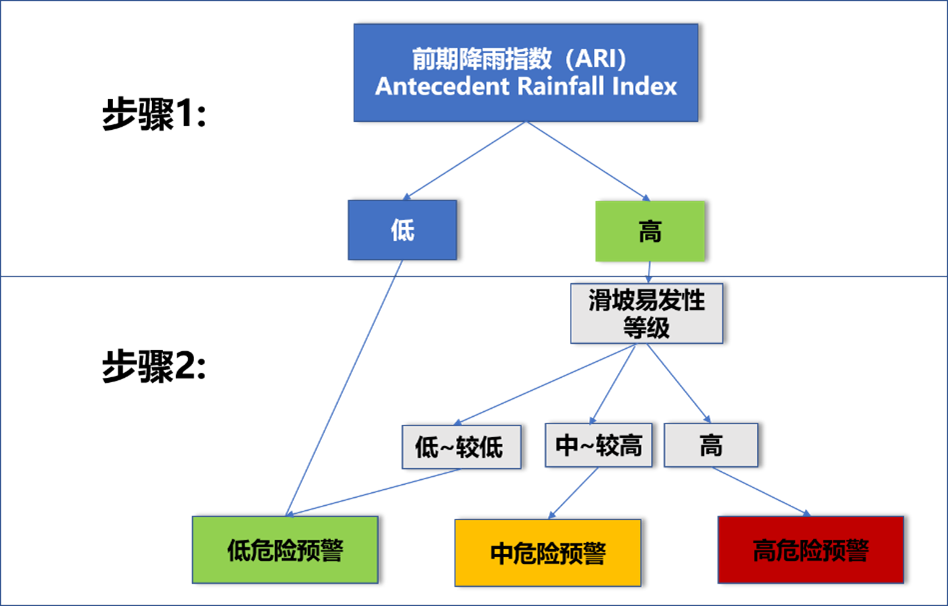
\includegraphics[width=10cm]{images/ari4nsfc.png}  
	\caption{技术路线图}
	\label{fig_ari4nsfc}
\end{figure*}

一般地，滑坡易发性评价结果分为5个等级，从低到高依次对于低易发区、较低易发区、中易发区、较高易发区和高易发区。
前期降雨指数的百分位数大于50，则可以认为是高指数等级。
对于研究区内任一点位，如果知道了它的前期降雨指数和滑坡易发性等级，即可利用图\ref{fig_ari4nsfc}所示的决策表计算它的风险等级。
\NsfcSection{4}{本项目的特色与创新之处；}{}

\subsection{提出了基于GEE云平台的滑坡危险性评价解决方案}

将GEE云平台引入到滑坡易发性和危险性评价当中，充分利用GEE云平台数据量大、处理能力强、数据更新快的优势，构建面向三峡库区全区的滑坡危险性动态评价方法体系，为三峡库区灾害管理提供可行性方案。

\subsection{将类别加权引入到滑坡易发性建模当中}

以往基于机器学习的滑坡易发性评价研究中，很少有研究关注非滑坡样本（负样本）的选取问题。
当尽可能多的选取了非滑坡样本，又会导致类别不均衡。
本研究针对滑坡样本类别不均衡的问题，使用类别加权的思想对传统随机森林方法进行改造，使之适用于处理类别不均衡的易发性评价问题，有望提高滑坡易发性评价模型的准确度和泛化能力。

\NsfcSection{5}{年度研究计划及预期研究结果}{（包括拟组织的重要学术交流活动、国际合作与交流计划等）。}

\subsection{年度研究计划}

（1）2022年：开展基础资料整理以及野外地质调查工作，厘清三峡库区滑坡地质灾害现状，收集研究区已有地质调查成果和历史遥感影像等。

（2）2023年：开展多源异构数据融合实验，探究适于研究区的不同尺度的融合策略；开发基于遥感大数据平台的地质灾害监测与风险评价系统；开展地质灾害变化检测与动态监测技术研究，开展野外验证工作。

（3）2024年：全面总结和分析项目研究成果，编制项目成果报告。完成项目审查以及成果报告修改完善工作，提交最终成果报告；撰写学术论文，申请软件著作权等。

\subsection{预期研究成果}

（1）建立基于遥感云平台的三峡库区地质灾害危险性动态评价方法技术体系； 

（2）提交技术研究报告； 

（3）发表学术论文 3 到 4 篇，其中至少 2 篇 SCI/EI 检索论文； 

（4）申请软件著作权 1 到 2 项。

%%%%%%%%%%%%%%%%%%%%%%%%%%%%%%%%%%%%%%%%%%%%%%%%%
\NsfcChapter{（二）研究基础与工作条件}{}

\NsfcSection{1}{研究基础}{（与本项目相关的研究工作积累和已取得的研究工作成绩）；}

申请人多年来一直从事遥感地质方面的研究工作，对于滑坡地质灾害危险性评价有着较为深入的研究。申请人已发表研究滑坡易发性中样本不均衡问题的论文一篇，申请基于GEE云平台的软件著作权一项，主持或参与多个地质灾害相关的项目，包括“863”项目——重大工程地质灾害快速监测与评估、地质环境遥感监测应用子系统、忠武管道地质灾害风险评估建模及系统研发等。
此外，项目的可行性也与以下几个方面息息相关：

（1）基于机器学习方法的滑坡易发性评价研究已经相对成熟，开源的机器学习算法及处理软件日益增加。

（2）大数据、云计算等技术的快速发展，面向科研工作者的免费的遥感大数据云平台如GEE、地质云等不断涌现。OSChina、Github、Gitee、StackOverFlow等社区聚集了大量的GEE云计算的使用者和爱好者，形成了极为健康的学习研究生态圈。

（3）研究者在三峡库区参加了大量的遥感地质解译和地质灾害风险评价工作，积累了大量的第一手资料，对库区典型地质灾害的分布和成因有着较为深入的理解。
综上所述，本项目的实施拥有良好的研究基础和较高的可行性。


\NsfcSection{2}{工作条件}{（包括已具备的实验条件，尚缺少的实验条件和拟解决的途径，包括利用国家实验室、国家重点实验室和部门重点实验室等研究基地的计划与落实情况）；}

从平台角度来说，项目依托单位东华理工大学“江西省放射性地学大数据技术工程实验室”可为开展遥感大数据融合分析、空间建模等提供软硬件支持和技术支持。
从团队角度来说，申请人所在研究团队学术氛围良好，工作条件优越，团队成员专业互补性强，能够保障项目的顺利实施。
从已有资料来说，申请人已经收集了大量的关于研究区大量资料，包括基础地质概况，地质调查数据，历史遥感影像和相关研究文献等。

\NsfcSection{3}{正在承担的与本项目相关的科研项目情况}{（申请人和项目组主要参与者正在承担的与本项目相关的科研项目情况，包括国家自然科学基金的项目和国家其他科技计划项目，要注明项目的名称和编号、经费来源、起止年月、与本项目的关系及负责的内容等）；}

无

\NsfcSection{4}{完成国家自然科学基金项目情况}{（对申请人负责的前一个已结题科学基金项目（项目名称及批准号）完成情况、后续研究进展及与本申请项目的关系加以详细说明。另附该已结题项目研究工作总结摘要（限500字）和相关成果的详细目录）。}

%%%%%%%%%%%%%%%%%%%%%%%%%%%%%%%%%%%%%%%%%%%%%%%%%

无

\NsfcChapter{（三）其他需要说明的问题}{}

\NsfcSection{1}{}{申请人同年申请不同类型的国家自然科学基金项目情况（列明同年申请的其他项目的项目类型、项目名称信息，并说明与本项目之间的区别与联系）。}

无

\NsfcSection{2}{}{具有高级专业技术职务（职称）的申请人或者主要参与者是否存在同年申请或者参与申请国家自然科学基金项目的单位不一致的情况；如存在上述情况，列明所涉及人员的姓名，申请或参与申请的其他项目的项目类型、项目名称、单位名称、上述人员在该项目中是申请人还是参与者，并说明单位不一致原因。}

无

\NsfcSection{3}{}{具有高级专业技术职务（职称）的申请人或者主要参与者是否存在与正在承担的国家自然科学基金项目的单位不一致的情况；如存在上述情况，列明所涉及人员的姓名，正在承担项目的批准号、项目类型、项目名称、单位名称、起止年月，并说明单位不一致原因。}

无

\NsfcSection{4}{}{其他。}

在2020年的青年科学基金申请中，评审专家给出了中肯且具有建设性的意见。
在2021年度青年科学基金的撰写过程中，本人认真考虑了评审专家提出的意见，并进行了深刻反思和逐条改正。
\end{document}
